\acp{HEMT} gehören zur Klasse der Feldeffekttransistoren, unterscheiden sich allerdings in ihrem Funktionsprinzip entscheidend von \acsp{JFET} und \acsp{MOSFET}.
Das Funktionsprinzip basiert auf einer Heterostruktur zweier Halbleiter mit unterschiedlich großen Bandlücken.
An der Grenzschicht zwischen einem stark n-dotierten Halbleiter mit großer Bandlücke (z.B. AlGaAs) und einem undotierten Halbleiter mit kleinerer Bandlücke (z.B. GaAs) kommt es zum band bending und es entsteht eine Struktur, wie sie in Abb. \ref{fig:HEMTBand} dargestellt ist.
Elektronen aus dem n-dotierten Material diffundieren in das Leitungsband auf der Seite des undotierten Materials.
Dadurch entsteht entlang der Grenzfläche ein 2D-Elektronengas.
Durch eine Spannung am Gate kann die Anzahl der Elektronen im Leitungsband beeinflusst werden.
Da sich die Leitungselektronen auf Seiten des undotierten GaAs befinden, kommt es seltener zu Coulomb-Streuung, was zu einer hohen Mobilität der Elektronen führt.
Daher stammt auch der Name von Transistoren dieser Art.\cite{HEMTFundamental, Mimura2002}

\begin{figure}[!b]
\begin{center}
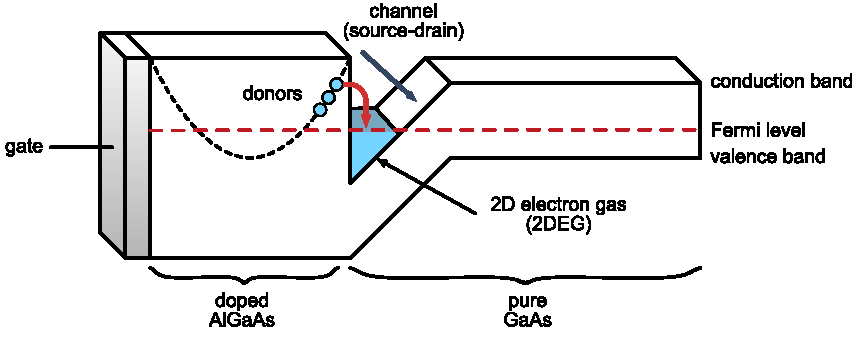
\includegraphics[scale=1]{./fig/HEMTBand.pdf}
\vspace{-0.5cm}
\caption{Bandstruktur eines typischen HEMTs.
Elektronen aus dem stark n-dotierten AlGaAs diffundieren in das undotierte GaAs und bilden dort ein 2D-Elektronengas.
Über die Gatespannung wird die Lage des Fermilevel und damit die Menge an Elektronen im Leitungsband variiert.\cite{Thomas2016}}
\label{fig:HEMTBand}
\end{center}
\end{figure}

Bisherige niederfrequente kryogene Verstärkerelektroniken basieren vorwiegend auf JFETs.
Die Technik von JEFTs stößt allerdings an zwei für diesen Anwendungsbereich entscheidende Grenzen.
Erstens frieren JFETs unter einer Temperatur von $\SI{100}{\kelvin}$ ein und werden idealerweise bei einer Temperatur von $\SI{130}{\kelvin}$ verwendet.
Daher ist entweder eine Heizung im Krysotaten notwendig oder lange Kabel zwischen Ausleseelektronik und Detektor, welche Auslesegeschwindigkeit und Signalqualität verringern.
Zweitens liegt das minimal mögliche Rauschen in der Größenordnung von $\SI{1}{\nano\volt\per\sqrt\hertz}$ bei einer Frequenz von $\SI{1}{\kilo\hertz}$\cite{HEMTYang2011}.
HEMTs und MOSFETs hingegen funktionieren selbst bei kryogenen Temperaturen.
Diese Arten von Transistoren wurden bisher allerdings nicht verwendet aufgrund ihres hohen niederfrequenten $1/f$-Rauschen.

Infolge aktueller Entwicklungen des \ac{CNRS} an der Universität Paris-Süd ist es gelungen HEMTs zu entwerfen, welche vielversprechende Eigenschaften aufweisen im Gegensatz zu handelsüblichen HEMTs.
Die Erste dieser Eigenschaften ist ein hervorragendes $1/f$-Rauschen von $\SI{0.46}{\nano\volt\per\sqrt\hertz}$ bei einer Frequenz von $\SI{1}{\kilo\hertz}$ und einer Temperatur von $\SI{4.2}{\kelvin}$.
Die Eingangskapazität liegt in der Größenordnung von $\SI{100}{\pico\farad}$, womit sie gut an die Detektorkapazität angepasst ist.
Zweitens liegt ihre benötigte Leistung in der Größenordnung von $\SI{30}{\mu\watt}$ deutlich unter der von JFETs.\cite{HEMTYang2011}
Dadurch ist es möglich eine größere Anzahl von Ionisationskanälen im Kryostaten zu installieren.
Zuletzt sind diese HEMTs zur Anwendung bei kryogenen Temperaturen ausgelegt.
Werden JFETs im Kryostaten verwendet, ist es notwendig eine Heizung einzubauen.
Diese erzeugt Schwarzkörperstrahlung, welche wiederum vom Detektor absorbiert werden kann.
Außerdem muss sie von der restlichen Anordnung isoliert werden. 
Die dazu verwendete Membran erzeugt zusätzliches niederfrequentes Rauschen durch ihre Schwingungen.




